%%%%%%%%%%%%%%%%%%%%%%%%%%%%%%%%%%%%%%
%%%%%%%%%%%%%%%%%%%%%%%%%%%%%%%%%%%%%%
% Do not edit the TeX file your work
% will be overwritten.  Edit the RnW
% file instead.
%%%%%%%%%%%%%%%%%%%%%%%%%%%%%%%%%%%%%%
%%%%%%%%%%%%%%%%%%%%%%%%%%%%%%%%%%%%%%



Our final data analysis example is an application of a Bayesian topic model to
population genetics. We consider a publicly available dataset from
\citet{galbusera:2000:thrush} that contains genotypes from 155 samples of an
endangered bird species, the Taita thrush. Individuals were collected from four
regions in southeast Kenya (Chawia, Mbololo, Ngangao, Yale), and each individual
was genotyped at seven micro-satellite loci. The four regions were once part of
a cohesive cloud forest that has since been fragmented by human development. For
this endangered bird species, understanding the degree to which populations have
grown genetically distinct is important for conservation efforts: well-separated
populations with little genetic diversity are particularly at risk of
extinction.  The goal of the analysis is to identify the presence of latent
populations, from which one can infer the population of origin for specific
loci, and estimate the degree to which populations are admixed in each
individual.


\subsubsection*{The model}

The data consists of consists of $\nindiv$ individuals genotyped at $\nloci$
loci. Let $\x_{\n\l\i}\in\{1, \ldots, J_\l\}$ be the observed genotype for
individual $\n$ at locus $\l$ and chromosome $\i$. $J_\l$ is the number of
possible genotypes at locus $\l$. For example, if the measurements are all
single nucleotides (A, T, C or G) then $J_\l = 4$ for all $\l$.

A latent population is characterized by the collection $\beta_k =
(\latentpop_{\k1}, \ldots, \latentpop_{\k\nloci})$ where
$\latentpop_{\k\l}\in\Delta^{J_\l - 1}$ are the latent frequencies for the $J_l$
possible genotypes at locus $\l$. Let $\z_{\n\l\i}$ be the assignment of
observation $\x_{\n\l\i}$ to a latent population. Notice that for a given
individual $\n$, different loci, or even different chromosomes at a given locus,
may have different population assignments. The distribution of
$\x_{\n\l\i}\in\{1, \ldots, J_\l\}$ arising from population $\k$ is
%
\begin{align*}
\p(\x_{\n\l\i} \vert \latentpop_{\k}) =
\categoricaldist{\x_{\n\l\i}\vert \latentpop_{\k\l}}.
\end{align*}

Unlike the previous models, we now have a stick-breaking process for each
individual. Draw sticks
%
\begin{align*}
\nu_{\n\k} \iid \pstick(\nu_{\n\k}) \quad \forall \n = 1, \ldots, \nindiv; \k = 1, 2, \ldots \infty.
\end{align*}
%
The prior assignment probability vector $\latentadmix_{\n} =
(\latentadmix_{\n1}, \latentadmix_{\n2}, \ldots)$, now unique to each
individual, is formed by the same stick-breaking construction as before,
%
\begin{align*}
\latentadmix_{\n\k} = \nu_{\n\k} \prod_{\k' < \k} (1 - \nu_{\n\k'}).
\end{align*}
%
The population assignment $\z_{\n\l\i}$ is drawn from the usual multinomial
distribution
%
\begin{align*}
p(\z_{\n\l\i} | \latentadmix_\n) = \prod_{k=1}^{\infty} \latentadmix_{\n\k}^{\z_{\n\l\i\k}}.
\end{align*}
%
In this genetics application, we call $\latentadmix_{\n}$ the \textit{admixture}
of individual $\n$.

This model is identical to fastSTRUCTURE, a model proposed in
\citet{pritchard:2000:structure, raj:2014:faststructure}, except that we replace
the Dirichlet prior in fastSTRUCTURE with an infinite stick-breaking process.
The result is a model similar to a hierarchical Dirichlet process for topic
modeling \citep{teh:2006:hdp}, but without the top-level Dirichlet process. In
addition, genotypes at genetic markers take the place of words in a document; in
lieu of inferring ``topics," we infer latent populations.

The variational approximation is mean-field as before, and all distributions are
conditionally conjugate except for the stick-breaking proportions, which remain
logit-normal. See \appref{app_structure} for further details.

\subsubsection*{The initial fit}

\todo{Say here what the $\alpha$ range should be and why.}

Since there are approximately four geographic regions we take $\alpha_0 = 3$,
corresponding to roughly four distinct populations {\em a priori}. We consider
the range $\alpha = 0.5, 1, \ldots 7$, corresponding to between two and seven
expected populations per individual under the GEM prior
(\eqref{prior_num_clusters}).

In the posterior with at $\alpha_0$, shown in \figref{stru_init_fit}, there
appear to be three dominant latent populations, which we arbitrarily label as
populations 1, 2, and 3. The inferred populations generally correspond with the
geographic regions: individuals from the Mbololo region have population 1 as
their dominant admixture proportion; individuals from the Ngangao are dominantly
population 2; individuals from the Chawia are admixed with populations 1, 2, and
3. The four individuals from Yale appear similar to individuals from the
Ngangao; this is not surprising given that the Yale region is geographically
located in proximity to the Ngangao region.  Our results with $\alpha_0$ are
qualitatively similar to those computed from the finite mixture model
fastSTRUCTURE fit with a heuristically chosen $K=3$ clusters in that we both
uncover three genetically distinct groups of individuals, corresponding with the
Chawia, Ngangao, and Mbololo geographical regions
\citet{pritchard:2000:structure}.

% The resulting inference from our BNP model is qualitatively similar to the
% results reported in \citet{pritchard:2000:structure} which used the
% fastSTRUCTURE model. Since fastSTRUCTURE is a finite mixture model based on $K$
% clusters, to select $K$, \citet{pritchard:2000:structure} ran fastSTRUCTURE with
% $K = 1, ..., 5$, and selected the $K$ that maximized a proxy for the posterior
% quantity $p(K | \x)$, under the assumption of a uniformly distributed prior on
% $K$. Their algorithm selected $K = 3$. At $\alpha_0 = 3$, the BNP model agrees
% with \citet{pritchard:2000:structure}


\begin{knitrout}
\definecolor{shadecolor}{rgb}{0.969, 0.969, 0.969}\color{fgcolor}\begin{figure}[!h]

{\centering 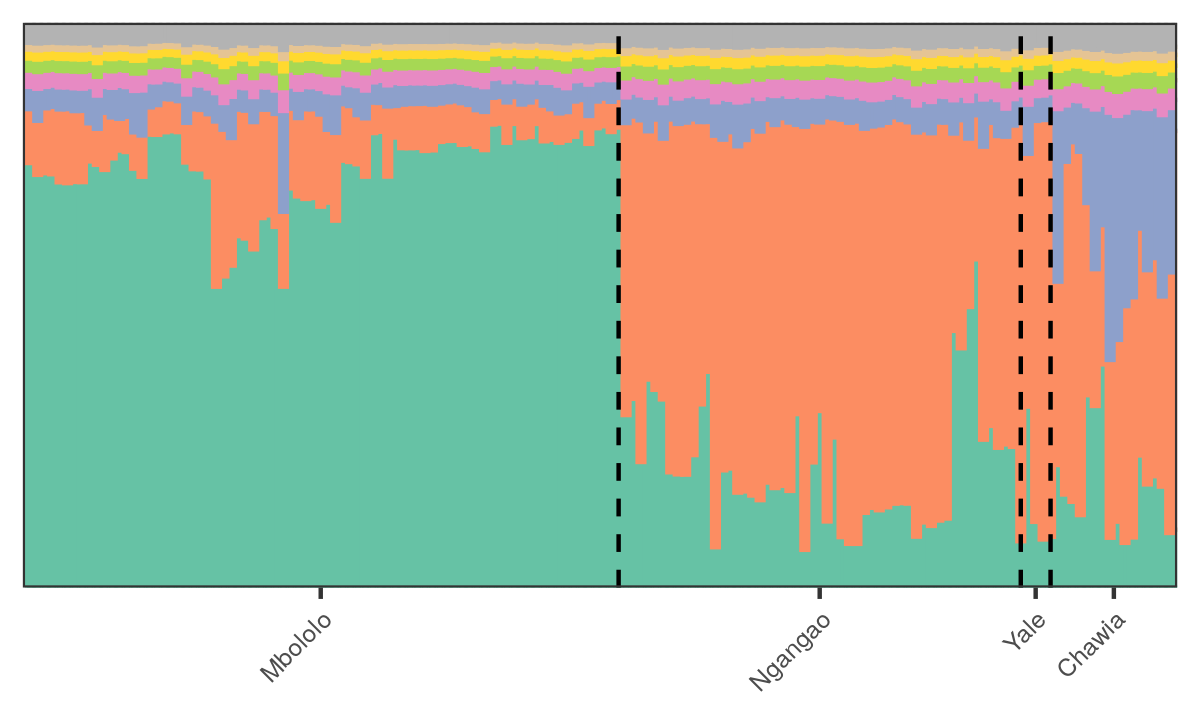
\includegraphics[width=0.980\linewidth,height=0.588\linewidth]{figure/stru_init_fit-1} 

}

\caption[The inferred individual admixtures at $\alpha_0 = 3$.
    Each vertical strip is an individual and each color
    a latent population.
    Lengths of colored segments represent the inferred admixture proportions.
    Individuals are ordered by the geographic region from which they were sampled
    (Mbololo, Ngangao, Yale, and Chawia).
    In the text, we refer to the green, orange, and purple latent populations
    as population 1, 2, and 3, respectively]{The inferred individual admixtures at $\alpha_0 = 3$.
    Each vertical strip is an individual and each color
    a latent population.
    Lengths of colored segments represent the inferred admixture proportions.
    Individuals are ordered by the geographic region from which they were sampled
    (Mbololo, Ngangao, Yale, and Chawia).
    In the text, we refer to the green, orange, and purple latent populations
    as population 1, 2, and 3, respectively. }\label{fig:stru_init_fit}
\end{figure}


\end{knitrout}

\subsubsection*{Quantities of interest}

\todo{Here, say what all the quantities of interest are and why}

Our posterior quantity of interest is the expected number of
in-sample populations (in this section, we will use ``populations" and ``clusters" interchangeably).
We consider a slightly more general definition than
\exref{vb_insample_nclusters_simple}: define
\begin{align*}
\gclusters(\eta)
&= \expect{\q(\z\vert\eta)}{\sum_{\k=1}^\kmax \ind{
\left(\sum_{\n=1}^{\nindiv}
\sum_{\l=1}^{\nloci}
\sum_{\i=1}^2
\z_{\n \l \i \k}\right) > \tau}},
\end{align*}
which is the expected number of populations in the data set that contains at least $\tau$ loci.
We allow the option of setting $\tau > 0$ in order to count only the populations that comprise a non-negligible fraction of the data set.
Other than the added parameter $\tau$, the only difference from
\exref{vb_insample_nclusters_simple} is that the summation
is now over individuals $n$, loci $\l$ and chromosomes $i$.

\todo{Reference the earlier def, and reference this def earlier}

\subsubsection*{Sensitivity of the number of populations to $\alpha$}

% $\gpop$ counts a population as present if they contain at least $\tau$ loci.
% When $\tau = 0$, $\gpop$ is equivalent to the expected in-sample number of clusters discussed in \secref{results_iris}, except the summation is now over individuals, loci, and chromosomes.

% At $\tau = 0$, $\gpop$ has a simple closed form expression as a function of the expectations of $\z_{\n \l \i \k}$;
% for $\tau > 0$, we resort to Monte Carlo estimates.
% Like the posterior quantity $\gclusterspred$ discussed in \secref{results_iris},
% we use the re-parameterization trick to sample from $\q(\z\vert\eta)$.
% This allows us to condition on fixed draws from a distribution that is independent of $\eta$ (in this case, the underlying distribution is $\mathrm{Uniform}[0, 1]$);
% these fixed draws are shared across every computation of $\gpop(\eta; \tau)$ below.

\todo{I think a major story here is that threshholding induces robustness.
We should make that point clear.}

\todo{Actually, I think we arguably don't care about the number of
populations for fastSTRUCTURE.  Could we possibly make this thresholding
point as part of the iris predictive example?}

The expected number of latent populations is sensitive to $\alpha$
(\figref{stru_alpha_nclusters}). Without any thresholding ($\tau = 0$), the
expected number of populations quickly increases as $\alpha$ increases; in fact,
it nearly saturates at $\kmax = 20$ when $\alpha = 7$. This sensitivity is
due to the fact that the non-thresholded quantity is highly dependent on
the behavior of small, nearly unoccupied populations; even though the
probability of a single locus belonging to these rare populations is small, the
probability that \textit{none} of the $\nindiv \times \nloci \times 2$ observed
genotypes belong to these rare populations is non-negligible.

This motivates the use of thresholding in reporting the number of populations.
We consider two thresholds, $\tau = 20$ and $\tau = 40$, corresponding to
approximately $2\%$ and $4\%$ of the total number of loci in the data set,
respectively. The thresholded estimates for the number of populations is still
moderately sensitive to the value of $\alpha$. When refitting the variational
approximation at $\alpha = 0.5, 1, \ldots, 7$, the thresholded quantities vary
between two and four latent populations.

The linearized variational parameters $\etalinglobal(\t)$ imperfectly captures
the results observed by refitting.
% We formed the linear approximation at
% $\alpha_0 = 3$ and computed $\gclusters(\etalinglobal(\alpha))$ for $\alpha =
% 0.5, 1, \ldots, 7$.
%For our choices of $\alpha$,
The linearized parameters and
the refitted parameters almost perfectly agree on values of $\gclusters$ with
$\tau = 0$. However, when $\tau = 20$, the linearized parameters underestimated
the true sensitivity of $\gclusters$ found by refitting. In particular, the
linearized parameters failed to produce the reduction to two latent populations
at $\alpha = 0.5$ observed in the refits.


\begin{knitrout}
\definecolor{shadecolor}{rgb}{0.969, 0.969, 0.969}\color{fgcolor}\begin{figure}[!h]

{\centering 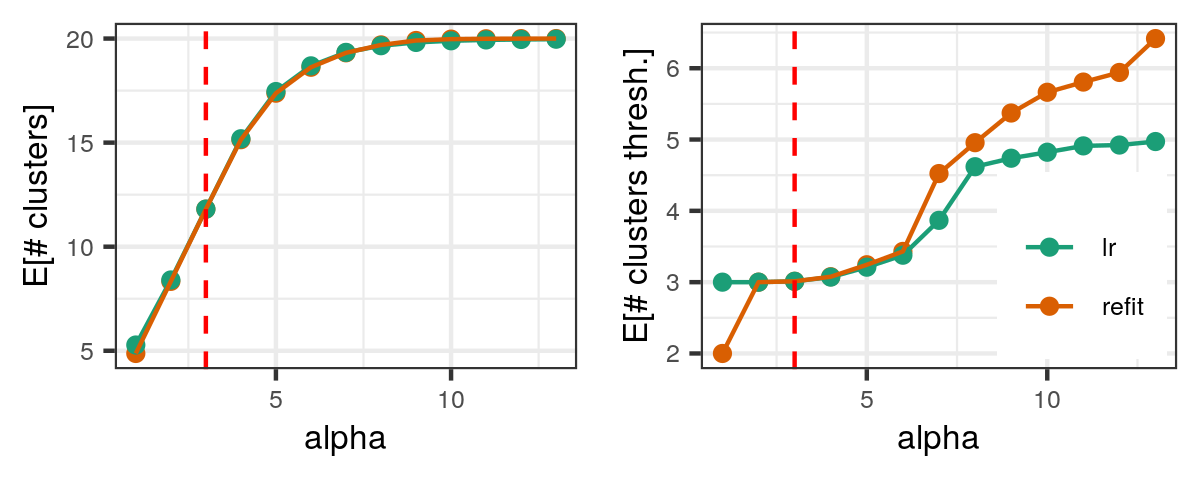
\includegraphics[width=0.980\linewidth,height=0.431\linewidth]{figure/stru_alpha_nclusters-1} 

}

\caption[The expected number of (thresholded)
    populations in the thrush data as $\alpha$ varies.
    We computed the linear approximation at $\alpha_0 = 3$, and
    we compare the
    results under the linearly approximated variational parameters with the
    results observed after refitting.
    Thresholds at $\tau = 20$ and $\tau = 40$ corresponding to
    approximately
    $2\%$ and $4\%$
    of the total number of loci in the data set, respectively]{The expected number of (thresholded)
    populations in the thrush data as $\alpha$ varies.
    We computed the linear approximation at $\alpha_0 = 3$, and
    we compare the
    results under the linearly approximated variational parameters with the
    results observed after refitting.
    Thresholds at $\tau = 20$ and $\tau = 40$ corresponding to
    approximately
    $2\%$ and $4\%$
    of the total number of loci in the data set, respectively. }\label{fig:stru_alpha_nclusters}
\end{figure}


\end{knitrout}

% We provide some more intuition concerning the thresholded estimate for the number of populations.
% The posterior quantity $\gclusters$ is closely related to the expected number of loci belonging to each population,
% defined as
% \begin{align*}
% \gloci(\eta; k)
% &= \expect{\q(\z\vert\eta)}{\sum_{n=1}^{\nindiv}
% \sum_{l=1}^{\nloci}
% \sum_{i=1}^2
% \z_{\n l i \k}}.
% \end{align*}
%
% \figref{stru_alpha_cluster_weights} plots $\gloci$ for the first six populations
% as $\alpha$ varies.
% The expected number of loci at the initial fit, $\gloci(\etaopt(\alpha_0); k)$,
% is at least 100 for populations $\k = 1, 2,$ and $3$ and
% less than
% ceiling(weights_alpha_init$weight[4])
% for the remaining populations.
% A sample of assignments $\z\sim \q(\z\vert\etaopt(\alpha_0))$ will
% almost always have at least $\tau$ loci allocated to populations 1, 2, and 3,
% while the allocations to each remaining population will almost always be below $\tau$, for either $\tau = 20$ or $\tau = 40$.
% Thus, at $\alpha = \alpha_0$ there then are clearly 3 populations by our definition of $\gclusters$, for either $\tau$.
%
% At $\alpha = 7$, the expected number of loci belonging to population 4
% increases to
% $sprintf('%.1f', weights_alpha_large$weight[4])$,
% a new population emerges above the threshold at $\tau = 20$.
% Both the linearized and the refitted variational parameters agree on this shift in allocation to population 4.
% On the other hand, under the refitted variational parameters at $\alpha = 0.5$,
% the expected number of loci belonging to population 3 decreases to
% $sprintf('%.1f', weights_alpha_small$weight[3])$,
% below the threshold $\tau = 20$.
% Thus, the expected number of latent populations with allocations above
% the threshold $\tau = 20$ decreases to two.
% The linearized parameters
% under-estimated this decrease in allocation to population 3, and
% therefore continued to estimate three latent populations even at $\alpha = 0.5$.




\subsubsection*{Sensitivity of individual admixtures to functional perturbations}

\todo{Move this up to the quantities of interest section}
Examining the inferred admixtures in \figref{stru_init_fit} provides clues into
the historical migration patterns of the genotyped individuals. For example,
while individuals collected from the Mbololo region are inferred to be admixed
primarily with population 1, several individuals from this region have
abnormally large admixture proportions of population 2. Conversely, while
individuals collected from the Ngangao region are admixed primarily with
population 2, a few of these individuals have abnormally large admixture
proportions of population 1. This suggests that some migration has occurred
between the Mbololo and Ngangao regions.

\todo{Left off here}

We evaluate the sensitivity of this conclusion to possible prior perturbations.
Consider the posterior statistic:
%
\begin{align*}
\gadmix(\eta; \mathcal{N}, k) =
 \expect{\q(\pi\vert\eta)}{\frac{1}{|\mathcal{N}|}\sum_{n\in\mathcal{N}}
\pi_{\n\k}},
\end{align*}
%
the average admixture proportion of population $\k$ in a set of
individuals $\mathcal{N}$.

We present results on three variations of $\gadmix$:
$\mathcal{N} = \{26, ..., 31\}$ and $k = 2$,
corresponding to the six individuals from the Mbololo region with outlying proportions of population 2;
$\mathcal{N} = \{125, ..., 128\}$ and $k = 1$,
corresponding to the four individuals from the Ngangao region with outlying proportions of population 1;
$\mathcal{N} = \{139, ..., 155\}$ and $k = 3$,
corresponding to all individuals from the Chawia region.
The first two posterior quantities relate to the inferred mixing between
Mbololo and Ngangao.
In the last case, we are studying the sensitivity of having a third latent
population present, a population which primarily appears in Chawia individuals.
\todo{Reference a figure here so it's clear what you're talking about}

In \figref{stru_func_sens}, we construct the worst-case negative perturbation
for each decreasing each of our three variant of $\gadmix$, in order to see
whether the biologically interesting patterns can be made to disappear
with different prior choices.

\todo{Make the text easier to match up with the picture, which doesn't
have the populations (Ngangao, \&c) labeled.  Right now it's hard to see
what's going on.}

\todo{I think this whole section could be easier to understand and much more
compact.  Basically just say that A is non-robust, B is robust, and on C
the linear approximation and refit disagree.  Then we investigate A more.}

Under the
linearized variational parameters $\etalinglobal(\t)$, the admixture proportion
of population 2 in the outlying Mbololo individuals is nearly halved.
The same quantity computed after refitting the model confirms the
sensitivity predicted by the linearized variational parameters.

 On the other
hand, the presence of population 1 in the outlying Ngangao individuals appears
to be insensitive even after this worst-case perturbation. The linearized and
the refitted variational parameters again agree on this conclusion. Finally, the
presence of population 3 in the Chawia individuals is anticipated to be
sensitive by the linearized parameters, as this admixture proportion steadily
decreases as $t\rightarrow 1$. However, under the refits, this admixture
proportion does not decrease steadily but rather levels off after $t = 0.5$.



\begin{knitrout}
\definecolor{shadecolor}{rgb}{0.969, 0.969, 0.969}\color{fgcolor}\begin{figure}[!h]

{\centering 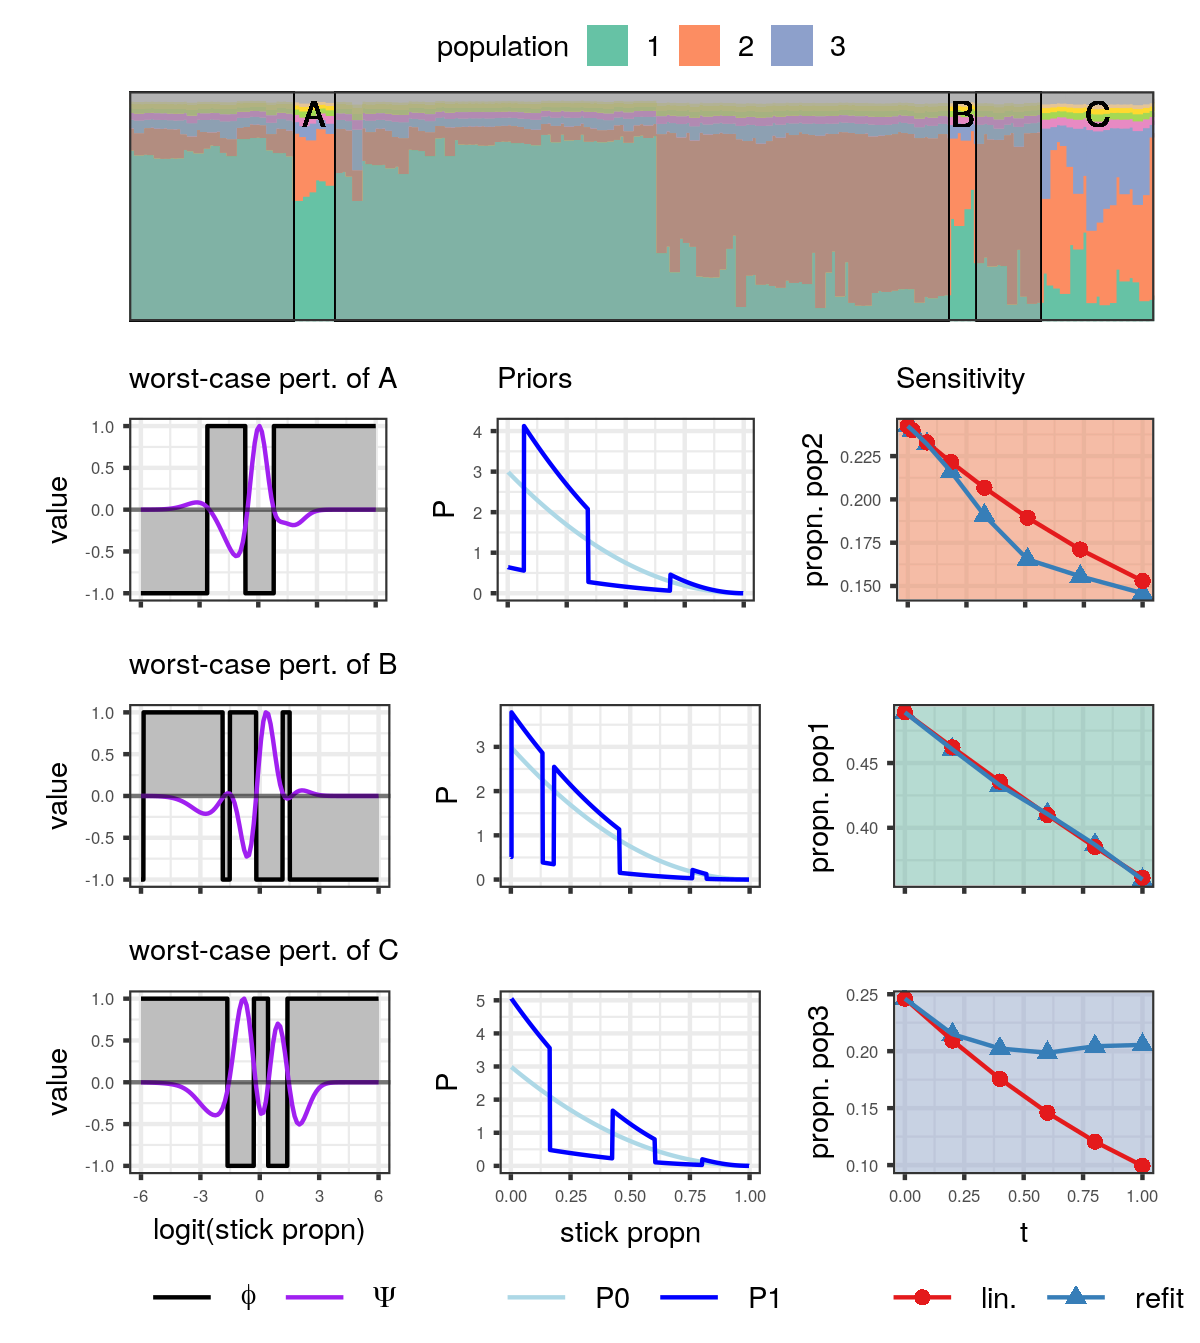
\includegraphics[width=0.980\linewidth,height=1.098\linewidth]{figure/stru_func_sens-1} 

}

\caption[Sensitivity of inferred admixtures for several outlying individuals.
     For individuals A,
     we examine the sensitivity of the admixture proportion of population 2.
     For individuals B,
     we examine the population 1 admixture
     For the individuals C, we examine the population 3 admixture.
     (Left column) The worst-case negative perturbation with unit $L_\infty$-norm
     in grey,
     plotted against the influence function in purple
     (scaled to also have $L_\infty$ norm equal to 1).
    (Middle column) The effect of the perturbation on the prior density.
    (Right column) Effects on the inferred admixture]{Sensitivity of inferred admixtures for several outlying individuals.
     For individuals A,
     we examine the sensitivity of the admixture proportion of population 2.
     For individuals B,
     we examine the population 1 admixture
     For the individuals C, we examine the population 3 admixture.
     (Left column) The worst-case negative perturbation with unit $L_\infty$-norm
     in grey,
     plotted against the influence function in purple
     (scaled to also have $L_\infty$ norm equal to 1).
    (Middle column) The effect of the perturbation on the prior density.
    (Right column) Effects on the inferred admixture. }\label{fig:stru_func_sens}
\end{figure}


\end{knitrout}

Our sensitivity analysis suggests that the inferred migration from Mbololo to
Ngangao based on the outlying Ngangao admixtures appears robust to our
stick-breaking prior. On the other had, the the outlying Mbololo admixtures
appears to be more sensitive to the stick-breaking prior, and conclusions about
migration from Ngangao to Mbololo may be dependent on prior choices.

\todo{Say something about the fact that these priors are maybe too
adversarial.}

\subsubsection*{Computation time}

The computational cost of linearizing the variational parameters is again
favorable compared with the cost of refitting (\tabref{stru_timing}).
Even though, for this model and dataset, the approximation matched refitting
less well, the influence function still provided a valuable guide for
identifying influential prior perturbations which could then be investigated
further with refitting.

% The linear approximation allows us to quickly explore all the
% functional perturbations presented here, and many more:
% computing the linearized variational parameters (including the Hessian inversion) $\etalinglobal$ takes about half a second for a given perturbation.
% On the other hand, refitting the model after a prior perturbation can take more than ten seconds.
% While exploring \textit{all} the possible functional perturbations is impossible, the linear approximation allows rapid exploration of the space of perturbations.
% Notice also that computing the influence function only takes half a second.
% As we have demonstrated, the influence function provides an informative guide
% for uncovering which perturbations might result in greater sensitivity than others.
% These perturbations can be more explored either by either linearizing in
% the direction of the perturbation, or by refitting.

\begin{table}[tb]
\centering
\caption{Compute time of results on the thrush dataset. Timing results
on perturbation $\phi$ are reported for the worst-case perturbation ``A"
in  \figref{stru_func_sens}. Timing on other considered $\phi$ are similar. }
\tablabel{stru_timing}
\begin{tabular}{|r|r|}
\hline
    & time (seconds) \\
    \hline
    Initial fit & 7 \\
    \hline
    Hessian solve for $\alpha$ sensitivity &
        0.32\\
    Linear approx. $\etalinglobal (\alpha)$ for $\alpha = 1, ..., 10$ &
        0.007\\
    Refits $\etaopt(\alpha)$ for $\alpha = 1, ..., 10$ &
        43\\
    \hline
    The influence function & 0.59\\
    Hessian solve for $\phi$ &
        0.38\\
    Linear approx. $\etalinglobal(\epsilon)|_{\epsilon = 1}$
      for $\phi$ &
        0.00085\\
    Refit $\etaopt(\epsilon)|_{\epsilon = 1}$
      for $\phi$ &
        13\\
    \hline
\end{tabular}
\end{table}

\subsection{Limitations of local sensitivity}

\todo{I agree that basically all of this section except for the figure could
go in the appendix and could be made much less wordy.  There are some other
examples of poor linear approximations in this section.  I think we should
make that a top-line takeaway of this experiment.}

In this final subsection,
we discuss some examples where
the linearized variational parameters $\etalin(t)$
are a poor substitute for the refitted variational parameters $\etaopt(t)$
(in this subsection, the only posterior quantities considered
are functions of global parameters, so we will not make a distinction
between $\etalin$ and $\etalinglobal$ here).
Naturally, the linearized parameters
$\etalin(t)$ will be a poor substitute for $\etaopt(t)$ when
the mapping $\t\mapsto\etaopt(\t)$ is highly nonlinear.
The examples discussed below use the STRUCTURE model and
dataset presented in \secref{results_structure}, and
we examine results after
the worst-case perturbation ``A" in \figref{stru_func_sens}.

Recall from \figref{stru_func_sens} that the linearized parameters
agreed with the refitted parameters
in predicting the diminished admixture proportion of population 2
in the outlying Mbololo individuals (individuals ``A")
at the perturbed prior $\p_1 = \p_0\exp(\phiworstcase)$.
However, while the linearized parameters were able to
capture the change in overall admixture proportion,
it does not perform uniformly well over all individual admixtures
(\figref{stru_func_sens_admix}).
For example, the admixture proportion of population 2 in individual $n = 25$
dramatically increased after refitting with the perturbed prior $\p_1$;
the linearized parameters failed to reproduce this change.


\begin{knitrout}
\definecolor{shadecolor}{rgb}{0.969, 0.969, 0.969}\color{fgcolor}\begin{figure}[!h]

{\centering 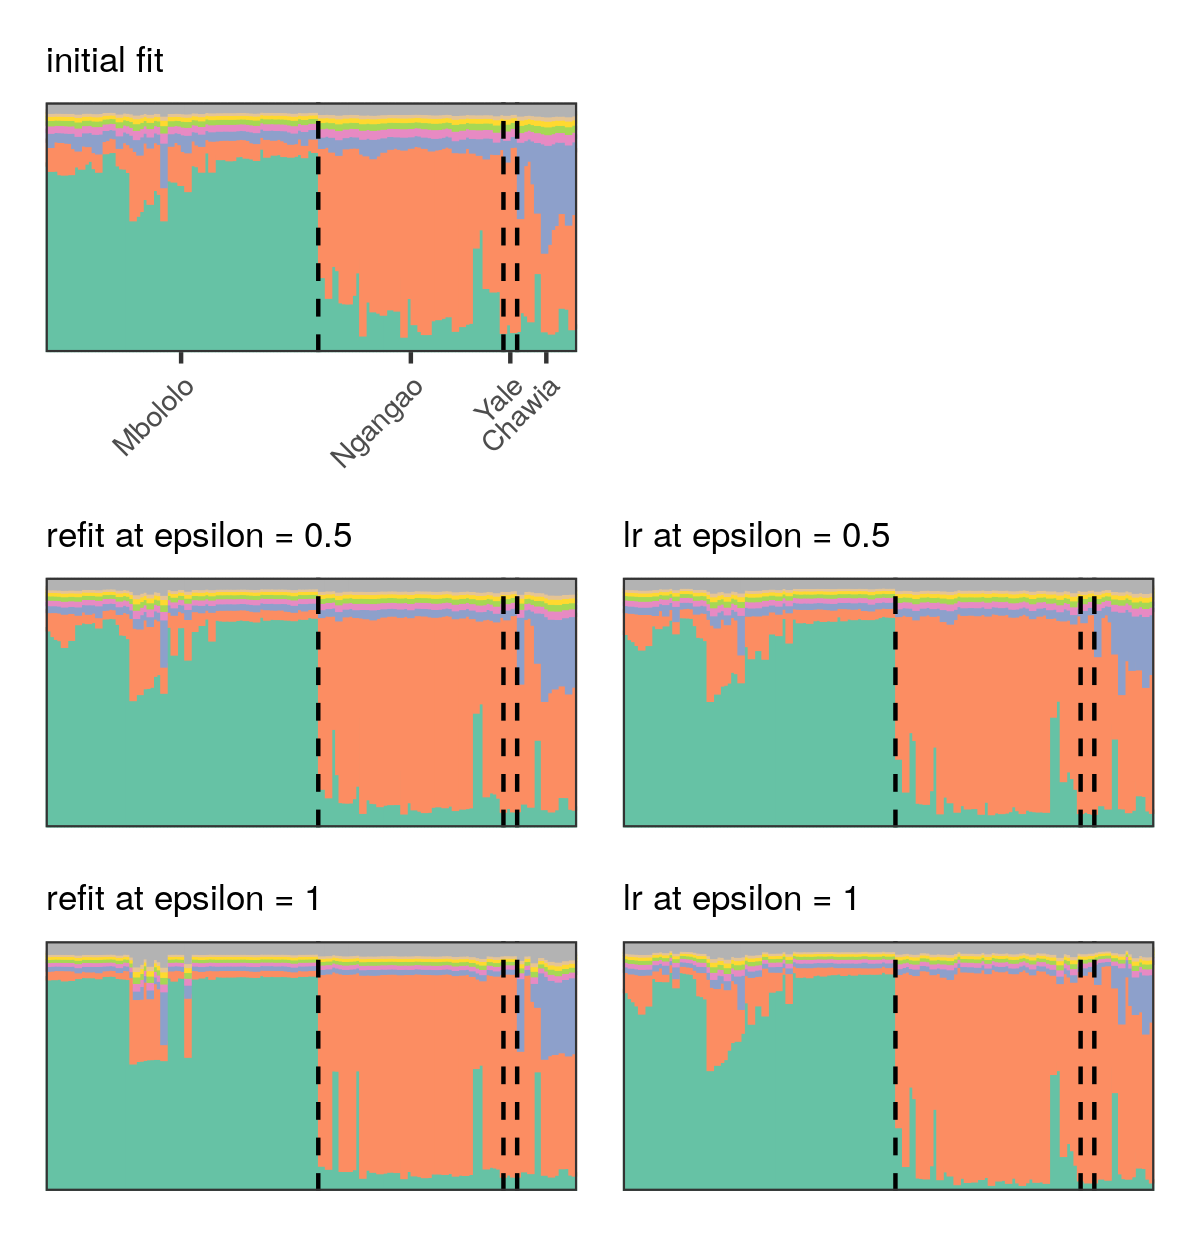
\includegraphics[width=0.980\linewidth,height=0.392\linewidth]{figure/stru_func_sens_admix-1} 

}

\caption{Inferred admixtures after the worst-case perturbation
     to individuals ``A" (see Figure~\ref{fig:stru_func_sens} for perturbation). }\label{fig:stru_func_sens_admix}
\end{figure}


\end{knitrout}

\figref{stru_lin_bad_example} examines individual $n = 25$ more closely.
The bottom row plots this individual's
admixture proportions as $\t$ varies from 0 to 1 in the perturbed prior
$\p(\nu\vert \t) = \p_0(\nuk)\exp(\t\phiworstcase(\nuk))$.
The linearized parameters poorly captured the change in admixture proportions observed after refitting, particularly
for populations 1 and 2, for values of $\t$ close to 1.
Even though we retain non-linearities
in the mapping from variational parameters to the posterior statistic,
for this perturbation, the mapping from prior parameter
$\t$ to the relevant variational parameters
is highly non-linear.
This latter mapping is what we linearize
and what causes our approximation to fail in this case.
Specifically, the variational location parameter on the first stick-breaking proportion is concave as a function of $\t$ ---
the location parameter increases for small $\t$,
then decreases as $\t\rightarrow1$.
However,
$\etalin(\t)$ linearizes the relationship between the location parameter and $\t$.
Therefore, the corresponding admixture mixture proportion of
population 1 is over-estimated under the linearized variational parameters.
Furthermore, because our linearized variational parameters
over-estimated the length of the first stick,
and the second admixture proportion is a product of the
remaining stick times the second stick-breaking proportion,
the linearized variational parameters then under-estimates
the admixture proportion of population 2.




\begin{knitrout}
\definecolor{shadecolor}{rgb}{0.969, 0.969, 0.969}\color{fgcolor}\begin{figure}[!h]

{\centering 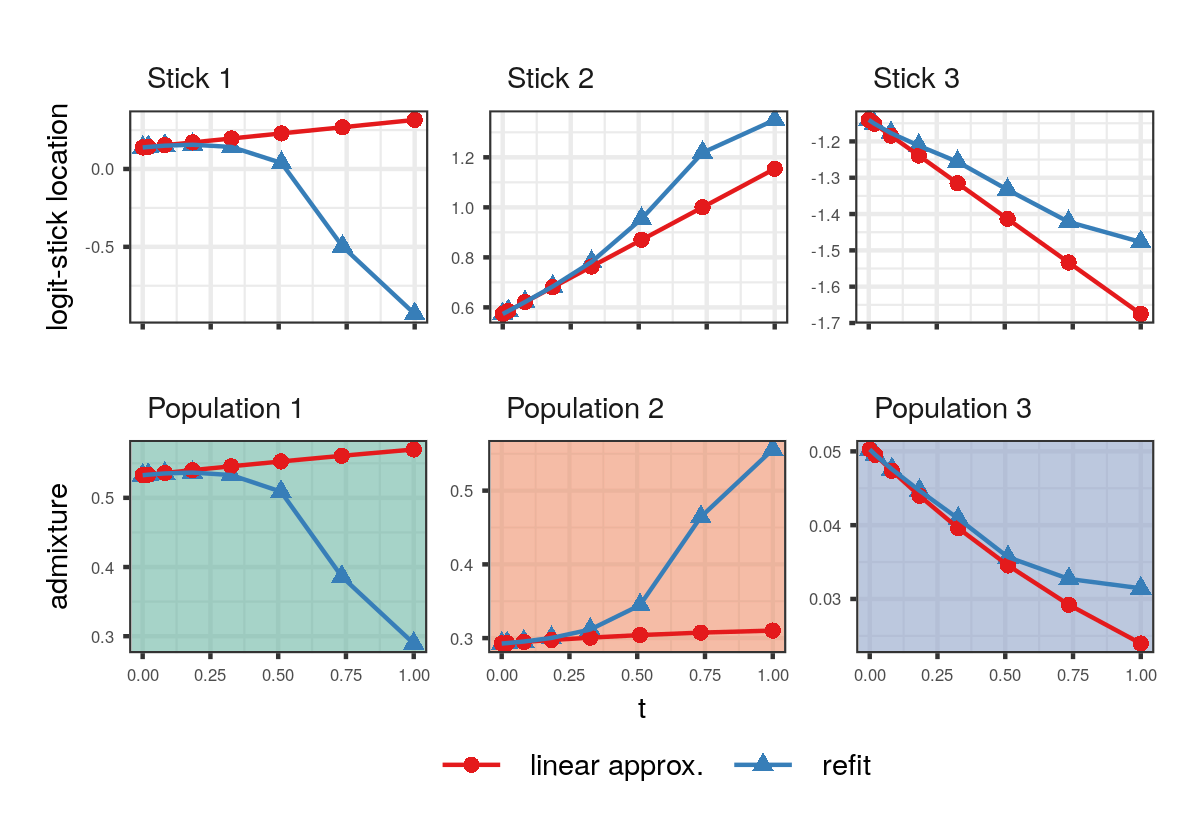
\includegraphics[width=0.980\linewidth,height=0.666\linewidth]{figure/stru_lin_bad_example-1} 

}

\caption[An individual $(\n = 26)$ for which
    the linearly approximated variational parameters
    poorly captured the
    change in admixture observed after refitting
    as $\t \rightarrow 1$.
    (Top row) the change in location parameter of the normally
    distributed logit-sticks, for the first three sticks.
    The response here is a variational parameter, so
    the approximation (red) is necessarily linear with respect to $\t$.
    (Bottom row) the change in the inferred admixtures for
    populations 1, 2, and 3]{An individual $(\n = 26)$ for which
    the linearly approximated variational parameters
    poorly captured the
    change in admixture observed after refitting
    as $\t \rightarrow 1$.
    (Top row) the change in location parameter of the normally
    distributed logit-sticks, for the first three sticks.
    The response here is a variational parameter, so
    the approximation (red) is necessarily linear with respect to $\t$.
    (Bottom row) the change in the inferred admixtures for
    populations 1, 2, and 3. }\label{fig:stru_lin_bad_example}
\end{figure}


\end{knitrout}



\figref{stru_fully_lin_example} shows a similar situation for individual $n = 74$.
The linearized variational parameters grossly over-estimated the length of the first stick,
resulting in the later admixture proportions being under-estimated.
The third admixture proportion was particularly poorly approximated under the linearized variational parameters.
Given the recursive nature of the relationship between admixtures and stick-breaking proportions, errors at early sticks affect later admixture proportions.
Fully linearizing the mapping $\t\mapsto\g(\etaopt(\t))$ to form the approximation
$\glin(t)$ avoids this problem.
In this example, $\glin(t)$ outperforms $\g(\etalin(t))$, with $\g$ being the admixture proportion of population 3.
In previous examples
(including the example in \figref{stru_lin_bad_example}),
computing $\g(\etalin(t))$, and thus retaining the non-linearities in the mapping from $\eta\mapsto\g(\eta)$,
does no worse, and is usually better,
than the fully linearized version, $\glin(\t)$---as can be seen by drawing tangent lines of the refitted curve at
$\alpha = \alpha_0$ or $t = 0$
in \figref{stru_alpha_nclusters, stru_lin_bad_example}.
It is likely that $\g(\etalin(t))$ outperforms $\glin(\t)$ for most posterior quantities, though as we see in \figref{stru_fully_lin_example},
this is not guaranteed to always be true.


% In the examples above, we only linearized the mapping $\epsilon \mapsto \etaopt(\epsilon)$.
% In most examples, we find that retaining the non-linearities from $\eta\mapsto g$ performed as well, or better than, fully linearizing the mapping from $\epsilon \mapsto \eta$.
% There are exceptions, as we discuss below.


\begin{knitrout}
\definecolor{shadecolor}{rgb}{0.969, 0.969, 0.969}\color{fgcolor}\begin{figure}[!h]

{\centering 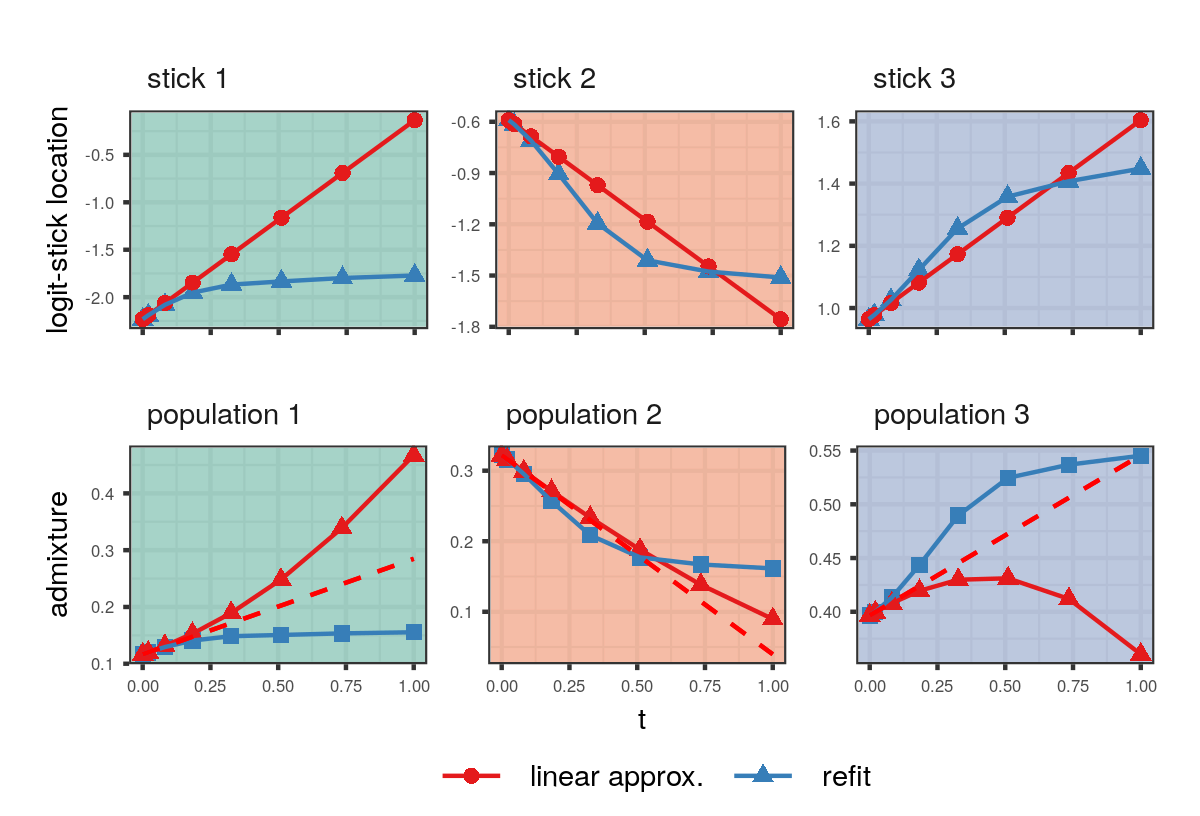
\includegraphics[width=0.980\linewidth,height=0.666\linewidth]{figure/stru_fully_lin_example-1} 

}

\caption[An example where
    linearizing the posterior quantity itself outperforms
    linearizing the variational parameters only.
    Shown are logit-stick location parameters (top row) and
    inferred admixtures (bottom row)
    for individual $n = 74$ and populations $k = 1, 2$ and $3$.
    Dashed red is the approximation $\glin(\t)$ formed by linearizing the
    inferred admixture $\expect{\q}{\pi_{\n\k}}$ with respect to prior
    parameter $t$.
    On the admixture proportion of population 3,
    $\glin(\t)$ outperforms $\g(\etalin(\t))$ (solid red)]{An example where
    linearizing the posterior quantity itself outperforms
    linearizing the variational parameters only.
    Shown are logit-stick location parameters (top row) and
    inferred admixtures (bottom row)
    for individual $n = 74$ and populations $k = 1, 2$ and $3$.
    Dashed red is the approximation $\glin(\t)$ formed by linearizing the
    inferred admixture $\expect{\q}{\pi_{\n\k}}$ with respect to prior
    parameter $t$.
    On the admixture proportion of population 3,
    $\glin(\t)$ outperforms $\g(\etalin(\t))$ (solid red). }\label{fig:stru_fully_lin_example}
\end{figure}


\end{knitrout}
